% This is the HU Berlin LaTeX template, optimized for R Markdown.

% -------------------------------
% --- PREAMBLE ---
% -------------------------------
\documentclass[a4paper,11pt]{article}

\usepackage{amsmath,amssymb,amsfonts,amsthm}    % Typical maths resource packages
\usepackage{graphicx}                           % Packages to allow inclusion of graphics
\usepackage[authoryear]{natbib}                 % literature reference style
\usepackage[bf]{caption}
\usepackage{textcomp}                           % For single quotes
\usepackage{floatrow}                           % For image and table position
\usepackage{booktabs}                           % For tables
% \usepackage[colorlinks=true]{hyperref}                           
% \usepackage[bottom]{footmisc}                   
\usepackage[bottom, flushmargin]{footmisc}                   % For footnotes
\usepackage[citebordercolor={0 1 0}]{hyperref}                           % For creating hyperlinks in cross references
\usepackage{footnotebackref}

% -------------------------------
% --- some layout definitions ---
% -------------------------------

% define topline
\usepackage[automark]{scrlayer-scrpage}
\pagestyle{scrheadings}
\automark{section}
\clearscrheadings
\ohead{\headmark}

% define citation style
\bibliographystyle{ecta}

% define page size, margin size
\setlength{\headheight}{1.1\baselineskip}
\voffset=-2cm
\hoffset=-3cm
\textheight24cm
\textwidth15.5cm
\topmargin1cm
\oddsidemargin3cm
\evensidemargin3cm
\setcounter{secnumdepth}{3}
\setcounter{tocdepth}{3}   
  \usepackage[parfill]{parskip} 

% define line spacing = 1.5
\renewcommand{\baselinestretch}{1.5}

% define position of graphics
\floatsetup[figure]{capposition=bottom}
\floatsetup[table]{capposition=bottom}
\floatplacement{figure}{ht}
\floatplacement{table}{ht}

% save thesis parameters for later
\newcommand{\thesistype}{Bachelor's Thesis}
\newcommand{\thesisauthor}{Daniel Kuhlen}
\newcommand{\thesisdate}{April 25, 2023}

% define tightlist to work with newer versions of pandoc
\providecommand{\tightlist}{%
  \setlength{\itemsep}{0pt}\setlength{\parskip}{0pt}}

% change spacing
\setlength {\parskip}{1em}

% Additional LaTeX parameters added in the YAML header of index.Rmd

% Added code to define CSLReferences environment
\usepackage{etoolbox}
\newlength{\cslhangindent}
\setlength{\cslhangindent}{1.5em}
\newenvironment{CSLReferences}[2] % #1: entry spacing, #2: hanging-indent width
 {\setlength{\cslhangindent}{#2\parindent}%
  \setlength{\parindent}{0pt}%
  \everypar{\setlength{\hangindent}{\cslhangindent}}\ignorespaces}
 {\par}


% --------------------------------------
% --------------------------------------
% --------------------------------------
% --- the structure the tex document ---
% ---  (this our recommendation) -------
% frontmatter:
%   - titlepage (mandatory),
%   - acknowledgement,
%   - abstract,
%   - table of contents (mandatory),
%   - list of abbreviations (not mandatory),
%   - list of figures (not mandatory),
%   - list of tables  (not mandatory) .
%
% body of the thesis (the structure of the thesis body is not mandatory, but the list of literature is mandatory):
%   - introduction,
%   - methods,
%   - data,
%   - results,
%   - conclusion,
%   - literature (mandatory),
%   - appendix (figures, tables).
%
% last page:
%   - declaration of authorship (mandatory).
% --------------------------------------
% --------------------------------------
% --------------------------------------
\begin{document}
% -------------------------------
% --- frontmatter: Title page ---
% -------------------------------
\thispagestyle{empty}
\begin{center}
  {\Large{\bf Sentiment Analysis of German Parliamentary Candidates' Tweets:
A Longitudinal Study on Electioneering Tone and Post-Election Shifts}} \vspace{0.5cm}

  Bachelor's Thesis submitted \\\vspace{0.5cm}
  to \\\vspace{0.5cm}
  \textbf{Prof.~Dr.~Jochen Müller} \\
  \textbf{Prof.~Dr.~Dont Know} \\\vspace{0.5cm}
  Humboldt-Universität zu Berlin \\
  Institut für Sozialwissenschaften \\
  Innenpolitik der Bundesrepublik Deutschland \\
   \vspace{1cm}

  \includegraphics[width=0.35\textwidth]{HU_Logo_small.png}
  
  by \\\vspace{0.5cm}
  \textbf{Daniel Kuhlen} \\
  (609376) \\
  
  \medskip
  \medskip
  in partial fulfillment of the requirements \\
  for the degree of \\
  \textbf{Bachelor of Arts in Sozialwissenschaften} \\\vspace{0.5cm}
  April 25, 2023
  
\end{center}
% ------------------------------------
% --- frontmatter: Acknowledgement ---
% ------------------------------------
\newpage
\hypertarget{acknowledgements}{%
\section*{Acknowledgements}\label{acknowledgements}}
\addcontentsline{toc}{section}{Acknowledgements}

I want to thank Andreas Küpfer for granting me access to his Twitter API,
which enabled the collection of tweets for this thesis. I also extend my
appreciation to Elias Koch, Linda Naddaf, Luna Strauch, Philipp Kuhlen, Vandross
Alage and Zorbey Özcan for their contributions to the manual coding of the tweets.
\pagestyle{plain}
\pagenumbering{roman}   % define page number in roman style
\setcounter{page}{1}    % start page numbering

% -----------------------------
% --- frontmatter: Abstract ---
% -----------------------------
\newpage
\hypertarget{abstract}{%
\section*{Abstract}\label{abstract}}
\addcontentsline{toc}{section}{Abstract}

In this study, I examine the tone of German parliamentary candidates' tweets before and after an election by employing sentiment dictionaries to analyze a large corpus of tweets spanning a one-year period. The objective is to uncover potential patterns and shifts in political communication on social media platforms during electioneering and post-election engagement. By doing so, I aim to contribute to the growing body of literature on political communication and sentiment analysis. This investigation offers valuable insights for political actors, campaign strategists, and scholars interested in the impact of digital communication on political behavior and public opinion.

% -----------------------------
% --- frontmatter: Contents ---
% -----------------------------
\newpage
\tableofcontents
\clearpage

% ----------------------------------------------------------
% --- frontmatter: List of Abbreviations (not mandatory) ---
% ----------------------------------------------------------
\newpage
\hypertarget{list-of-abbreviations}{%
\section*{List of Abbreviations}\label{list-of-abbreviations}}
\addcontentsline{toc}{section}{List of Abbreviations}
\begin{tabular}{rp{0.2cm}lp{1cm}rp{0.2cm}l}
    CPI     & &  Consumer Price Index   & & ETF     & &  Equity Traded Funds  \\
    ETH     & &  Eat the Horse          & & XLM     & &  Xetra Liquidity
\end{tabular}
% ----------------------------------------------------
% --- frontmatter: List of Figures (not mandatory) ---
% ----------------------------------------------------
\newpage
\listoffigures
\addcontentsline{toc}{section}{List of Figures}

% ---------------------------------------------------
% --- frontmatter: List of Tables (not mandatory) ---
% ---------------------------------------------------
\newpage
\listoftables
\addcontentsline{toc}{section}{List of Tables}

% -------------------------------
% --- main body of the thesis ---
% -------------------------------
\newpage
\pagestyle{plain}       
\setcounter{page}{1}    % start page numbering anew
\pagenumbering{arabic}  % page numbers in arabic style

\hypertarget{introduction}{%
\section{Introduction}\label{introduction}}

\newpage

\hypertarget{theory}{%
\section{Theory}\label{theory}}

\hypertarget{literature-review}{%
\subsection{Literature Review}\label{literature-review}}

\hypertarget{hypotheses}{%
\subsection{Hypotheses}\label{hypotheses}}

\newpage

\hypertarget{methodology}{%
\section{Methodology}\label{methodology}}

\hypertarget{identification-strategy}{%
\subsection{Identification Strategy}\label{identification-strategy}}

\hypertarget{unit-of-analysis}{%
\subsubsection{Unit of Analysis}\label{unit-of-analysis}}

\hypertarget{treatment-and-outcome}{%
\subsubsection{Treatment and Outcome}\label{treatment-and-outcome}}

\hypertarget{assumptions}{%
\subsubsection{Assumptions}\label{assumptions}}

\newpage

\hypertarget{data}{%
\section{Data}\label{data}}

To address the research questions at hand, a dataset comprising 876548 tweets from from 1345 candidates and 43 party accounts affiliated with the SPD, CDU, FDP, Linke, Grüne and AfD is utilized. The dataset captures all tweets by these accounts within a one year time frame before and after the election for the 20th German Bundestag (federal parliament) on the September 26, 2021.

In order to collect the data for analysis, I first obtained the Twitter handles for all relevant accounts using two hand curated datasets: (\protect\hyperlink{ref-konigEPINetzTwitterPoliticians2022}{König 2022}) and (\protect\hyperlink{ref-saltzerTwitterAccountsCandidates2021}{{``Twitter Accounts of Candidates in the {German} Federal Election 2021 ({GLES}){Twitter-Accounts} Der {Kandidierenden} Zur {Bundestagswahl} 2021 ({GLES})''} 2021}) These datasets not only provide the Twitter handles for candidates, politicians, and parties but also offer valuable metadata, including party affiliation, age, and other relevant information. Using the Twitter handles I then scraped the Twitter Data with the academic license to the platforms API.

\hypertarget{variables}{%
\subsection{Variables}\label{variables}}

\hypertarget{results}{%
\section{Results}\label{results}}
\begin{itemize}
\item
  Organize material and present results.
\item
  Use tables, figures (but prefer visual presentation):
  \begin{itemize}
  \item
    Tables and figures should supplement (and not duplicate) the text.
  \item
    Tables and figures should be provided with legends.
  \item
    \emph{Figure \ref{fig:graph} shows how to include and reference graphics.
    The graphic must be labelled before. Files must be in \textbf{.eps} format. You
    can do this really easily in R Markdown with \texttt{knitr::include\_graphics()}}!
  \item
    Figures can be referenced with \texttt{\textbackslash{}@ref(fig:\textless{}name\textgreater{})}, where \texttt{\textless{}name\textgreater{}} is the
    name of the code chunk.
  \end{itemize}
\end{itemize}
\begin{figure}

{\centering 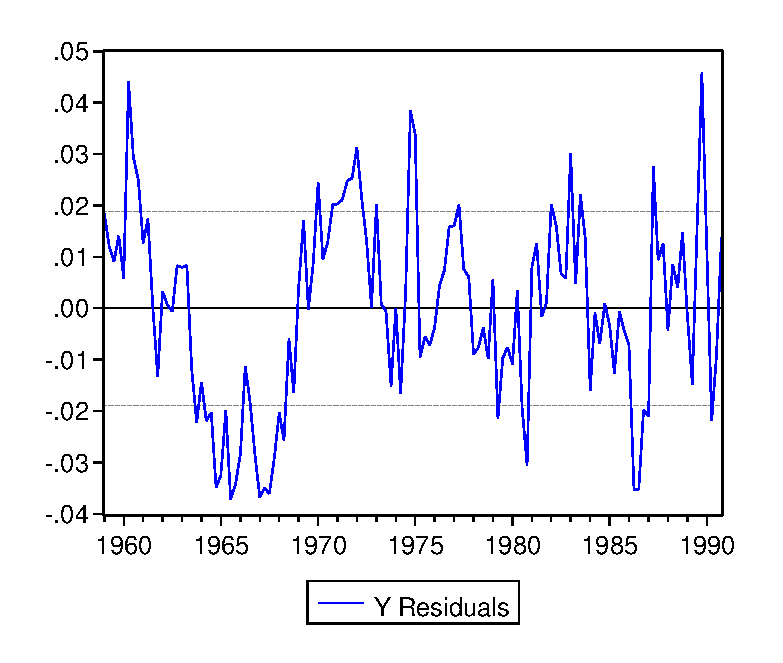
\includegraphics[width=0.5\linewidth]{figures/graph} 

}

\caption{Estimated residuals from model XXX. ...}\label{fig:graph}
\end{figure}
\begin{itemize}
\item
  Tables and graphics may appear in the text or in the appendix, especially if
  there are many simulation results tabulated, but is also depends on the study
  and number of tables resp. figures. The key graphs and tables must appear in
  the text!
\item
  R Markdown can also supports math equations just like \emph{LaTeX}!
  \begin{itemize}
  \item
    \emph{Equation \eqref{eq:SpecDens} represents the ACs of a stationary
    stochastic process:}
    \begin{equation}
            f_y(\lambda) = (2\pi)^{-1} \sum_{j=-\infty}^{\infty}
                           \gamma_j e^{-i\lambda j}
                         =(2\pi)^{-1}\left(\gamma_0 + 2 \sum_{j=1}^{\infty}
        \gamma_j \cos(\lambda j)\right)
                                       \label{eq:SpecDens}
    \end{equation}
    \emph{where \(i=\sqrt{-1}\) is the imaginary unit, \(\lambda \in [-\pi, \pi]\) is the
    frequency and the \(\gamma_j\) are the autocovariances of \(y_t\).}
  \item
    Equations can be referenced with \texttt{\textbackslash{}@ref(eq:\textless{}name\textgreater{})}, where name is defined
    by adding \texttt{(\textbackslash{}\#eq:\textless{}name\textgreater{})} in the line immediately before \texttt{\textbackslash{}end\{equation\}}.
  \end{itemize}
\end{itemize}
\hypertarget{review-of-results}{%
\subsection{Review of Results}\label{review-of-results}}
\begin{itemize}
\item
  Do the results support or do they contradict economic theory ?
\item
  What does the reader learn from the results?
\item
  Try to give an intuition for your results.
\item
  Provide robustness checks.
\item
  Compare to previous research.
\end{itemize}
\hypertarget{conclusion}{%
\section{Conclusion}\label{conclusion}}
\begin{itemize}
\item
  Give a short summary of what has been done and what has been found.
\item
  Expose results concisely.
\item
  Draw conclusions about the problem studied. What are the implications of your
  findings?
\item
  Point out some limitations of study (assist reader in judging validity of
  findings).
\item
  Suggest issues for future research.
\end{itemize}
\newpage

\hypertarget{references}{%
\section*{References}\label{references}}
\addcontentsline{toc}{section}{References}

\noindent

\setlength{\parindent}{-0.5cm}
\setlength{\leftskip}{0.5cm}
\setlength{\parskip}{8pt}

\hypertarget{refs}{}
\begin{CSLReferences}{1}{0}
\leavevmode\vadjust pre{\hypertarget{ref-konigEPINetzTwitterPoliticians2022}{}}%
König, Tim. 2022. {``{EPINetz Twitter Politicians} 2021.''} {GESIS Data Archive}. \url{https://doi.org/10.7802/2415}.

\leavevmode\vadjust pre{\hypertarget{ref-saltzerTwitterAccountsCandidates2021}{}}%
{``Twitter Accounts of Candidates in the {German} Federal Election 2021 ({GLES}){Twitter-Accounts} Der {Kandidierenden} Zur {Bundestagswahl} 2021 ({GLES}).''} 2021. {GESIS Data Archive}. \url{https://doi.org/10.4232/1.13790}.

\end{CSLReferences}
\indent
\setlength{\parindent}{17pt}
\setlength{\leftskip}{0pt}
\setlength{\parskip}{0pt}

\newpage

\appendix

\hypertarget{appendix}{%
\section{Appendix}\label{appendix}}

Here goes the appendix!

\hypertarget{figures}{%
\subsection{Figures}\label{figures}}
\begin{figure}

{\centering 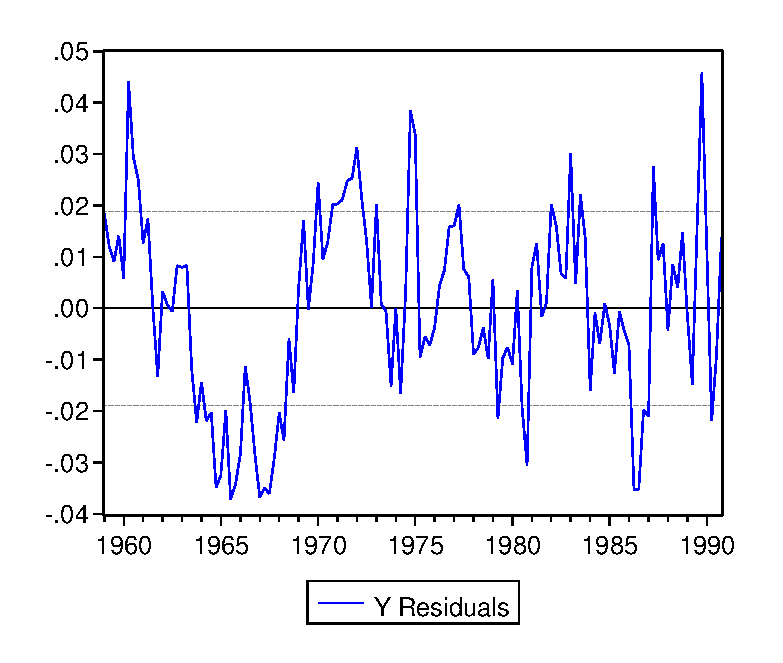
\includegraphics[width=0.5\linewidth,]{figures/graph} 

}

\caption{Estimated residuals (2) from model XXX. ...}\label{fig:graph2}
\end{figure}
\hypertarget{tables}{%
\subsection{Tables}\label{tables}}
\begin{table}[ht]
    \begin{center}
        {\footnotesize
        \begin{tabular}{l|cccccccccc}
        \hline \hline
                        & 3m    & 6m    & 1yr   & 2yr   & 3yr   & 5yr   & 7yr   & 10yr  & 12yr  & 15yr   \\
            \hline
                Mean   & 3.138 & 3.191 & 3.307 & 3.544 & 3.756 & 4.093 & 4.354 & 4.621 & 4.741 & 4.878  \\
                Median & 3.013 & 3.109 & 3.228 & 3.490 & 3.680 & 3.906 & 4.117 & 4.420 & 4.575 & 4.759  \\
                Min    & 1.984 & 1.950 & 1.956 & 2.010 & 2.240 & 2.615 & 2.850 & 3.120 & 3.250 & 3.395  \\
                Max    & 5.211 & 5.274 & 5.415 & 5.583 & 5.698 & 5.805 & 5.900 & 6.031 & 6.150 & 6.295  \\
                StD    & 0.915 & 0.919 & 0.935 & 0.910 & 0.876 & 0.825 & 0.803 & 0.776 & 0.768 & 0.762  \\
            \hline \hline
        \end{tabular}}
    \end{center}
    \caption{Detailed descriptive statistics of location and dispersion for
    2100 observed swap rates for the period from
    February 15, 1999 to March 2, 2007. Swap rates measured as 3.12 (instead of 0.0312).}
    \label{tab:apptable}
\end{table}
\newpage

% change rmd_files in `_bookdown.yml` files to determine order
% note that references and appendix are also contained here.

% --------------------------------------------
% --- last page: Declaration of Authorship ---
% --------------------------------------------

\newpage
\thispagestyle{empty}
\hypertarget{declaration-of-authorship}{%
\section*{Declaration of Authorship}\label{declaration-of-authorship}}

I hereby confirm that I have authored this \thesistype{} independently and
without use of others than the indicated sources. All passages which are
literally or in general matter taken out of publications or other sources are
marked as such.
\vspace{1cm}

Berlin, \thesisdate{}
\vspace{3cm}

. . . . . . . . . . . . . . . . . . . . . . . . . . . . . . .
\vspace{0.1cm}

\thesisauthor{}


\end{document}
